% ........................................................................... %

In the previous chapters, we have both introduced the model of \emph{timed protocols} and presented our approach for analyzing the pairwise compatibility or replaceability of two timed protocol instances. The set of flexible protocol compatibility and replaceability analysis classes that we presented can each be characterized by combining timed protocol operators. Yet, the decidability and closure properties of those operators remain to be studied ($\intersop$, $\compop$, $\diffop$, $\sqsubseteq$ and $\equiv$). To do that, we study those issues on protocol timed automata by reusing and adapting existing work from the theory of timed automata. As we will see, the case of $\intersop$ and $\compop$ is easy while the remaining operators pose more challenges. Indeed, they all rely on the ability to complement protocol timed automata, which is difficult as they have $\varepsilon$-labeled switches that cannot be removed in the general case. One strong theoretical contribution of this work is given here through the closure under complementation of protocol timed automata. This is the first class of timed automata with $\varepsilon$-labeled switches where this is possible.\\

This chapter is divided in two sections. The first one works at the protocol timed automata level and studies the closure of this class under intersection, then complementation. The second section leverages the results on protocol timed automata and translates them to timed protocols, leading to the decidability and closure properties of the timed protocol operators $\intersop$, $\compop$, $\diffop$, $\sqsubseteq$ and $\equiv$.

% ........................................................................... %

\section{Results in protocol timed automata}

% ........................................................................... %

We first study the intersection of protocol timed automata, then complementation. For each operator, the structure of the sections is identical: we give a procedure, an example and a theorem for the closure under the considered operator.

% ........................................................................... %

\subsection{Intersection of protocol timed automata}

% ........................................................................... %

The protocol timed automata intersection procedure extends the classical construction on timed automata \cite{RADLD94}, which in turns already extends the construction on (untimed) automata \cite{Hopcroft79}. We start by giving the procedure followed by an example. Then, we introduce a theorem for the closure of protocol timed automata under intersection.

\begin{procedure}
Given two protocol timed automata $A_1 = (L_1, L^0_1, L^f_1, X_1 \cup Y_1, E_1, \Sigma_1)$ and $A_2 = (L_2, L^0_2, L^f_2, X_2 \cup Y_2, E_2, \Sigma_2)$, the intersection $A_3 = A_1 \cap A_2$ (with $A_3 = (L_3, L^0_3, L^f_3, X_3 \cup Y_3, E_3, \Sigma_3)$) is built through the following steps.
\begin{enumerate}
  
  \item The locations are $L_3 = L_1 \times L_2$, the initial location is $L_3^0 = (L^0_1, L^0_2)$ and the final locations are $L_3^f = \left\lbrace (l_1, l_2) \;|\; l_1 \in L^f_1,\; l_2 \in L^f_2 \right\rbrace$.
  
  \item Two switches $e_1 = (l_1, g_1, a_1, r_1, l_1') \in A_1$ and $e_2 = (l_2, g_2, a_2, r_2, l_2') \in A_2$ are synchronized if and only if $a_1 = a_2 \neq \varepsilon$, producing a new switch $e_1e_2$ which is added to $A_3$: $e_1e_2 = ((l_1, l_2), g_1 \wedge g_2, a_1, \{x_{e_1e_2}\}, (l_1', l_2'))$ (this introduces a new clock $x_{e_1e_2}$ in $A_3$).
  
  \item $\varepsilon$-labeled switches are first added to $A_3$ with their guard being freed of $\permits$ clauses.
  We consider their guards to be disjunction-free (i.e., a $\varepsilon$-labeled witch whose guard is disjunctive is equivalent to several $\varepsilon$-labeled switches with conjunctive guards). 
  For each pair of $\varepsilon$-labeled switches
  $$
  \left\lbrace \begin{array}{l}
  
  e_1 = (l_1, (x_1 = k_1) \wedge g_1, \varepsilon, r_1, l_1') \in A_1 \\
  
  e_2 = (l_2, (x_2 = k_2) \wedge g_2, \varepsilon, r_2, l_2') \in A_2 \\
  
  \end{array} \right.
  $$
  we add the following switches to $E_3$:
  $$
  \left\lbrace \begin{array}{l}
  
  e_1e_\varepsilon = \left( (l_1, l_2), (x_1 = k_1) \wedge g_1 \wedge ((x_2 \neq k_2) \vee \neg g_2), \varepsilon, \{ x_{e_1e_\varepsilon} \}, (l_1', l_2) \right) \\
  
  e_\varepsilon e_2 = \left( (l_1, l_2), (x_2 = k_2) \wedge g_2 \wedge ((x_1 \neq k_1) \vee \neg g_1), \varepsilon, \{ x_{e_\varepsilon e_2} \}, (l_1, l_2') \right) \\
  
  e_1e_2 = \left( (l_1, l_2), (x_1 = k_1) \wedge (x_2 = k_2) \wedge g_1 \wedge g_2 , \varepsilon, \{ x_{e_1e_2} \}, (l_1', l_2') \right) \\
  
  \end{array} \right.
  $$
  
  \item With the set of clocks in $A_3$ being $X \cup Y$ as per definition, make sure that for each location $l$ offering at least one $\varepsilon$-labeled switch, a clock $y_l \in Y$ is reset on all of the incoming switches to $l$.
  
  \item For each location $l \in A_3$, compute the $\permits$ clauses.
  
  \item The guards in $A_3$ need to be rewritten to refer to the clocks of the switches of $A_3$ as they still refere to those of $A_1$ and $A_2$ at this step. A map is maintained between each clock $x_{e}$ of $A_1$ or $A_2$ and the set of clocks $\{ x_{e,e1}, x_{e,e2}, x_{e3,e}, \cdots \}$ that correspond to the switches $\{ (e,e1), (e, e2), \cdots, \}$ that were generated from $e$. Given a guard $g$ of a switch in $A_3$, a clause $(x_e \;\#\; k)$ of $g$ is rewritten as a disjunction $(x_{e,e1} \;\#\; k) \vee (x_{e,e2} \;\#\; k) \vee \cdots$. Diagonal constraint clauses in $g$ are also rewritten in a similar fashion using the mappings of its two clocks.
  
\end{enumerate}
\end{procedure}

\begin{figure}[htbp]
  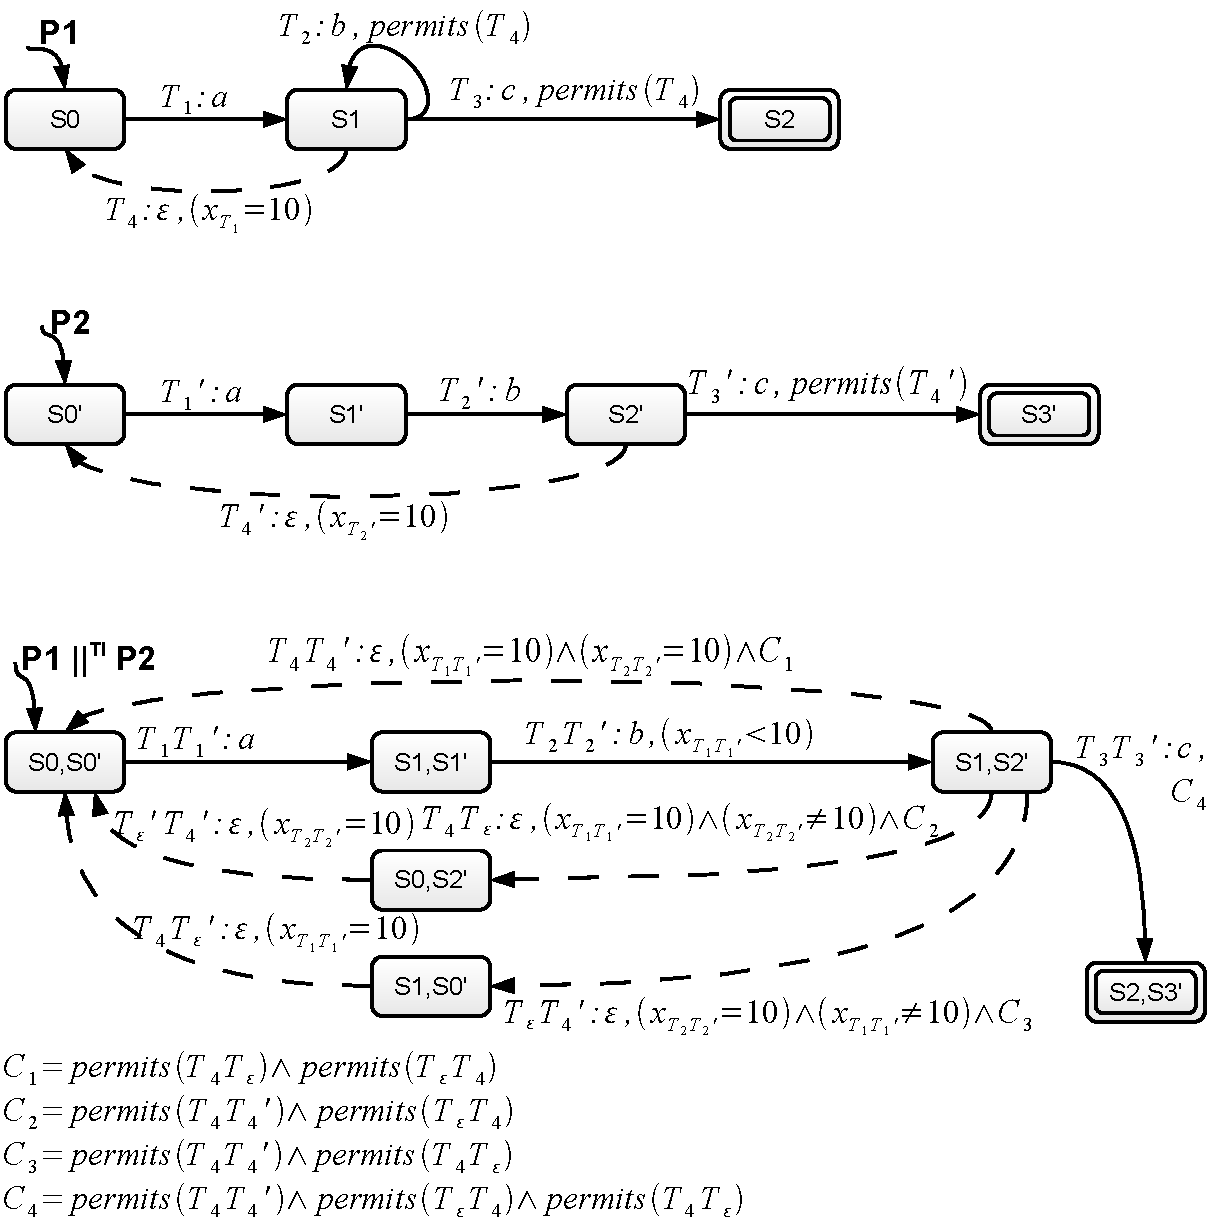
\includegraphics[width=\textwidth]{content/protocol-operators/sample-intersection}
  \caption{Two protocol timed automata $P_1$ and $P_2$ as well as their intersection $P_1 \intersop P_2$.}
  \label{fig:sample-intersection}
\end{figure}

Figure~\ref{fig:sample-intersection} gives an example of two protocol timed automata $P_1$ and $P_2$ as well as their intersection $P_1 \intersop P_2$. We deliberately abused notation for the sake of clarity by referring to transition identifiers in the $\permits$ functions instead of referring to guards.\\

Please note that in this procedure we remove the existing $\permits$ clauses in the guards as new ones are computed.
An extra step when actually implementing this procedure in a programming language would be to prune the locations that are not reachable from the initial location and the \emph{``deadlock''} locations, i.e., the non-final locations $l$ such that they don't provide any outgoing switch. The guards rewriting step is necessary because a switch of one of the input protocol timed automata may yield more than one switch in the resulting one. An example is the $T_4$ switch on $P_1$ from Figure~\ref{fig:sample-intersection} as it generates $T_4T_4'$, $T_4T_\varepsilon$, $T_\varepsilon T_4'$, $T_4T_\varepsilon'$ and $T_\varepsilon' T_4'$ in $P_1 \intersop P_2$. \\

Compared to the classic timed automata intersection procedure, the protocol timed automata intersection has the following differences.
\begin{enumerate}
  
  \item Clocks assignment remains ``under control'' to match the protocol timed automata requirement of having at most two clocks reset per transition. The classical timed automata intersection construction would simply combine the set of clocks from both input timed automata and merge the clocks in the reset sets of each switch. For example on Figure~\ref{fig:sample-intersection}, $T_2T_2'$ would reset the clock assigned to $T_2$ and the one assigned to $T_2'$.
  
  \item \MInvoke semantics are enforced in the intersection by computing new $\permits$ clauses (the $\permits$ clauses of the input timed automata guards are discarded).
  
\end{enumerate}

Protocol timed automata are closed under intersection (e.g., $A_3 = A_1 \cap A_2$ still belongs to the class).

\begin{theorem}
The class of protocol timed automata is closed under intersection.
\label{thm:closure-intersection}
\end{theorem}

The proof of the previous theorem is given on page~\pageref{proof:closure-intersection}.

% ........................................................................... %

\subsection{Complementation of protocol timed automata}

% ........................................................................... %

While protocol timed automata intersection is useful for characterizing timed protocol intersection and parallel composition, the complementation plays a critical role when it comes to characterizing the protocol difference and subsumption operators. Moreover, complementation of timed automata has traditionally been a difficult problem. Indeed, few classes of timed automata are closed under complementation \cite{RAPM04}.\\

We compute the complement of a protocol timed automaton using the following procedure which is derived from the one for deterministic timed automata as given in \cite{RADLD94}, with the difference lying in the presence of $\varepsilon$-transitions.

\begin{procedure}
Given a protocol timed automaton $A$, we denote by $A^*$ its \emph{complete} automaton which is build as follows.
\begin{enumerate}

  \item A location $q$ is added to $A^*$ whose role is to act as a \emph{rejection} location: given any timed word $w$ defined over $\overline{\mathcal{L}(A)}$, the execution of $w$ over $A^*$ goes to the location $q$ as soon as an input symbol yields to a word which is not in $\mathcal{L}(A)$. Hence, any timed word $w$ defined over the alphabet of $A$ has a (unique) execution over $A^*$.

  \item For each location $l$ of $A$ (this includes $q$) and for each word $a$ of the alphabet, a transition
  $$ 
  e = \left( 
    l, \left( g \bigwedge\limits_{1 \leq i \leq n} \permits(g_{\varepsilon i}) \right), a, \{ x_e \}, q
    \right)
  $$ is added where:
  \begin{enumerate}
    \item $g$ is defined as the negation of the disjunctions\footnote{e.g., given 2 $a$-labeled switches with guards $g_1$ and $g_2$, $g = \neg(g_1 \vee g_2)$} of the guards\footnote{For each guard, we do not take into account the clauses that are obtained through the $\permits$ function.} of the other $a$-labeled transitions from $l$, and
    \item each $g_{\varepsilon i} = (x_i = k_i) \wedge g_{\varepsilon i}'$ appears in the guard of the $i$-th $\varepsilon$-labeled switch from $l$, given that $l$ offers $n \geq 0$ of such switches.
  \end{enumerate}

\end{enumerate}
As in \cite{RADLD94}, the complement $\overline{A}$ of $A$ is deduced from $A^*$ by inverting the final and the normal locations due to the fact that every timed word $w \in \mathcal{L}(A)$ has a unique run over $A$.
\end{procedure}

\begin{figure}[htbp]
  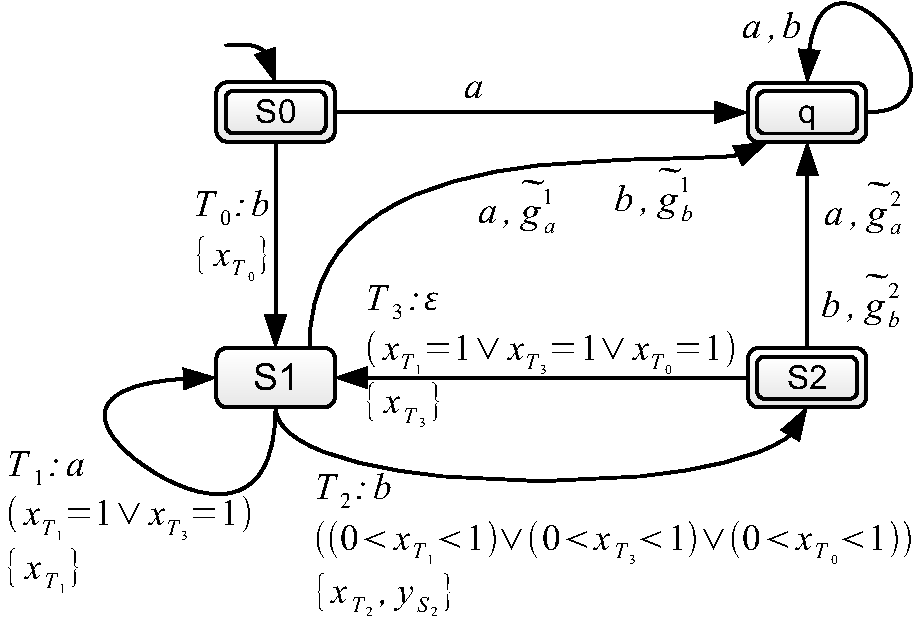
\includegraphics[width=\textwidth]{content/protocol-operators/complement-precise-time}
  \caption{The complement of the protocol timed automaton of Figure~\ref{fig:precise-time} (with drawing shortcuts).}
  \label{fig:complement-precise-time}
\end{figure}

As an example, we give on Figure~\ref{fig:complement-precise-time} the complement of the protocol timed automaton of Figure~\ref{fig:precise-time}. For the sake of clarity, we took some shortcuts in the drawing by combining the switches to $q$ that have been added from the same source location. The added guards are as follows:
\begin{itemize}
  
  \item $\widetilde{g_a^1} = (x_{T_1} \neq 1) \wedge (x_{T_3} \neq 1)$
  
  \item $\widetilde{g_b^1} = (x_{T_1} = 0 \vee x_{T_1} \geq 1) \wedge (x_{T_3} = 0 \vee x_{T_3} \geq 1) \wedge (x_{T_0} = 0 \vee x_{T_0} \geq 1)$
  
  \item $\widetilde{g_a^2} = \widetilde{g_b^2} = $
  
    $\left(
     (x_{T_1} < 1) \vee \left( (x_{T_1} > 1) \wedge (x_{T_1} - y_{S_2} > 1) \right)
    \right)
    \bigwedge$    
    
    $\left(
      (x_{T_3} < 1) \vee \left( (x_{T_3} > 1) \wedge (x_{T_3} - y_{S_2} > 1) \right)
    \right)    
    \bigwedge$
    
    $\left(
      (x_{T_0} < 1) \vee \left( (x_{T_0} > 1) \wedge (x_{T_0} - y_{S_2} > 1) \right)
    \right)$
  
\end{itemize}

As mentioned in the next theorem (a proof is given on page~\pageref{proof:closure-complement}), protocol timed automata are closed under complementation. This is a very interesting result, not only because it allows us to properly implement a timed protocol operator such as the difference, but also because the introduction of $\varepsilon$-labeled switches strictly increases expressiveness over (indeterministic) timed automata. Interestingly, previous results would not have suggested that protocol timed automata would be closed under complementation.

\begin{theorem}
The class of protocol timed automata are closed under complementation.
\label{thm:closure-complement}
\end{theorem}

The proof is given on page~\pageref{proof:closure-complement}.

% ........................................................................... %

\section{Results for timed protocol operators}

% ........................................................................... %

The closure properties of protocol timed automata under intersection and complementation allows to derive the following theoretical results for timed protocol operators.
The result on the intersection and parallel composition operators is straightforward.

\begin{corollary}
Timed protocols are closed under $\intersop$, $\compop$ and $\diffop$.
\end{corollary}

Both $\intersop$ and $\compop$ operators are based on the intersection using a different matching of the messages depending on their polarities:
\begin{itemize}
  
  \item in the case of $\intersop$, two messages match when they have the same name and polarity (e.g., $a(+)$ and $a(+)$)
  
  \item in the case of $\compop$, two messages match when they have the same name but a different polarity (e.g., $a(+)$ and $a(-)$).
  
\end{itemize}

The result on the difference operator derives from the closure of protocol timed automata under both intersection and complementation. Indeed, $\mathcal{P}_1 \diffop \mathcal{P}_2$ is equivalent to $\mathcal{P}_1 \intersop \overline{\mathcal{P}_2}$, hence timed protocol are also closed under difference.

\begin{corollary}
The timed protocol comparison operators $\sqsubseteq$ and $\equiv$ are decidable.
\end{corollary}

This comes from the closure under complementation and intersection as well as from the decidability of the reachability problem \cite{RADLD94}. Checking if $L(A_1) \subseteq L(A_2)$ is equivalent to checking whether $L(A_1 \cap \overline{A_2}) = \emptyset$ or not. A technique for checking emptiness of protocol timed automata using the UPPAAL model checker is discussed in the appendix at page~\pageref{chap:uppaal-pta}.

% ........................................................................... %